\documentclass[12pt]{article}

\usepackage[T1]{fontenc}
\usepackage[utf8]{inputenc}
\usepackage[russian]{babel}

% page margin
\usepackage[top=2cm, bottom=2cm, left=2cm, right=2cm]{geometry}

\usepackage{graphicx}

% AMS packages
\usepackage{amsmath}
\usepackage{amssymb}
\usepackage{amsfonts}
\usepackage{amsthm}

% blackboar lettering
\usepackage{dsfont}
\usepackage{bbm}

\usepackage{fancyhdr}
\pagestyle{fancy}
% modifying page layout using fancyhdr
\fancyhf{}
\renewcommand{\sectionmark}[1]{\markright{\thesection\ #1}}
\renewcommand{\subsectionmark}[1]{\markright{\thesubsection\ #1}}

\rhead{\fancyplain{}{\rightmark }}
\cfoot{\fancyplain{}{\thepage }}

\usepackage{titlesec}

% for appendix environment
\usepackage[titletoc,toc,title,page]{appendix}

\newcommand{\lb}{\left(}
\newcommand{\rb}{\right)}

\newcommand{\mf}{\mathbf}

\usepackage{dsfont}

\newcommand{\bbE}{\mathds{E}}
\newcommand{\bbS}{\mathds{S}}
\newcommand{\bbP}{\mathds{P}}

\newcommand{\mL}{\mathcal{L}}
\newcommand{\mN}{\mathcal{N}}
\newcommand{\intty}{\int\limits_{-\infty}^{+\infty}}

\usepackage{bbm}

\newcommand{\bbI}{\mathds{I}}
\newcommand{\bba}{\mathbbm{a}}
\newcommand{\bbA}{\mathds{A}}

\usepackage{algorithm}
\usepackage[noend]{algpseudocode}

\titleformat{\section}{\bfseries}{\thesection.}{1em}{}
\titleformat{\subsection}{\normalfont\itshape\bfseries}{\thesubsection.}{0.5em}{}

\title{Дискретные сигналы и преобразование Фурье}
\date{}

\begin{document}

\maketitle

Время принципиально по-разному проявляется в непрерывных и дискретных сигналах, что приводит к разному представлению частот в непрерывном и дискретном случаях. Продемонстрируем это на примере. Пусть нам дан список пар значений сигнала, и нас просят определить частоту колебания, подходящее для описания сигнала. Мы отложим на графике дискретные значения и, скажем, угодаем синусоидальную волну в них. Мы можем сказать, что волна повторяется каждые 20 точек, то есть ее период составляет 20 точек. Но использовать это соображение для нахождения частоты колебания невозможно, имея лишь значения сигнала. Для того, чтобы определить частоту колебания нам необходимо, например, время между значениями сигнала $t_s$. Пусть нам дано $t_s = 0.05$ мс, в таком случае период колебания равен $20 \cdot 0.05$ мс $= 1$ мс. Т.к. частота колебания обратна периоду, то получаем частоту колебания $1$ кГц. 

\section{Неопределенность сигнала в частотной области}

\begin{figure}[!ht]
	\centering
	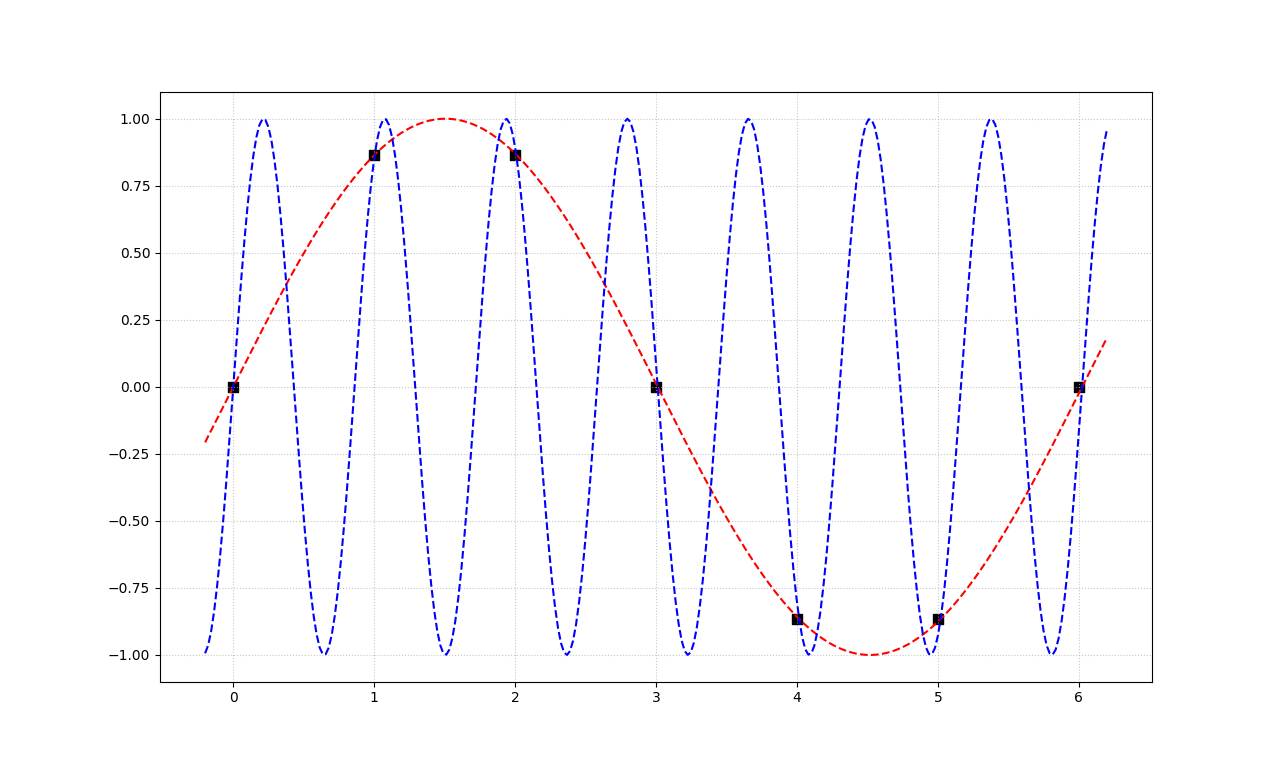
\includegraphics[width = 0.85\linewidth]{../pictures/aliasing.png}
	\caption{Несколько синусоид, соответствующих дискретному сигналу}
\end{figure}

\end{document}
